\documentclass{article}

% NeurIPS 2026 Workshop double-blind formatting (official style)
\usepackage[main]{neurips_2026_local}  % NeurIPS 2026 Main Track, double-blind

\usepackage[utf8]{inputenc}
\usepackage[T1]{fontenc}
\usepackage{amsmath,amssymb}
\usepackage{booktabs}
\usepackage{graphicx}
%\usepackage{microtype}  % disabled: requires scalable fonts
\usepackage{xcolor}
\usepackage{url}
\usepackage{hyperref}
\usepackage{pifont}
\usepackage{xspace}
\usepackage{tabularx}
\usepackage{natbib}
% Compatibility shims for unavailable packages
\newcommand{\makecell}[2][]{\shortstack[l]{#2}}
% adjustbox shim: just pass through (table* environment already full-width)
\newenvironment{adjustbox}[1]{}{}
% multirow shim: just use the content
\newcommand{\multirow}[3]{#3}
% enumitem shim: accept optional argument but ignore it
\makeatletter
\def\enumerate{\@ifnextchar[{\@enumerate@opt}{\begin{list}{\arabic{enumi}.}{\usecounter{enumi}\setlength{\itemsep}{1pt}\setlength{\topsep}{2pt}}}}
\def\@enumerate@opt[#1]{\begin{list}{\arabic{enumi}.}{\usecounter{enumi}\setlength{\itemsep}{1pt}\setlength{\topsep}{2pt}}}
\def\endenumerate{\end{list}}
\def\itemize{\@ifnextchar[{\@itemize@opt}{\begin{list}{\textbullet}{\setlength{\itemsep}{1pt}\setlength{\topsep}{2pt}}}}
\def\@itemize@opt[#1]{\begin{list}{\textbullet}{\setlength{\itemsep}{1pt}\setlength{\topsep}{2pt}}}
\def\enditemize{\end{list}}
\makeatother

\setlength{\emergencystretch}{2em}

\hypersetup{
  colorlinks=true,
  linkcolor=black,
  citecolor=black,
  urlcolor=black,
  pdfauthor={Anonymous Authors},
  pdftitle={MORPH-DA: A Mutation-Grounded Benchmark for Metamorphic Verification of Data-Analysis Agents}
}

\newcommand{\morph}{\textsc{Morph-DA}\xspace}
\newcommand{\wep}{wrong-but-executable program}
\newcommand{\weps}{wrong-but-executable programs}
\newcommand{\taskSpec}{\texttt{TaskSpec}\xspace}
\newcommand{\cmark}{\ding{51}}
\newcommand{\xmark}{\ding{55}}
\newcommand{\pp}{\,pp}
\newcommand{\secref}[1]{Section~\ref{#1}}
\newcommand{\figref}[1]{Figure~\ref{#1}}
\newcommand{\tabref}[1]{Table~\ref{#1}}

\title{\morph: A Mutation-Grounded Benchmark for\\
Metamorphic Verification of Data-Analysis Agents}
\author{Anonymous Authors}

\begin{document}
\normalsize
\maketitle

\begin{abstract}
Data-analysis agents increasingly generate and execute Python programs, but successful execution does not establish that the program implemented the requested filters, aggregation, grouping, denominator, or date window. We introduce \morph, a benchmark and environment-grounded runtime verifier for such \emph{wrong-but-executable} programs. The verifier is gold-answer-free at runtime but specification-conditioned: it receives a structured analytical specification, never the reference output, and checks operator-aware metamorphic relations by rerunning the same program on controlled data transformations. The benchmark contains 101 compositional tasks and 563 validated, non-equivalent semantic mutants. \morph detects 364/563 faults (64.7\%, 95\% task-clustered CI [58.4, 70.5]) versus 9/563 for universal robustness checks ($p=9.4\times10^{-79}$). Re-executing each seed-42 agent program unchanged on held-out data seeds reveals that 13--16 programs per model (20--26\% of apparently correct programs) are \emph{accidental corrects}. With this corrected ground truth, \morph obtains 79--89\% precision and 67--79\% recall on executable programs, with 8--21\% false-positive rate. A one-step repair study on 91 wrong programs yields 12.1\% fixes from relation-specific feedback versus 5.5\% from generic feedback. These results position metamorphic execution as a complementary, zero-additional-LLM-call verifier rather than a correctness certificate.
\end{abstract}

\section{Introduction}
\label{sec:intro}

LLM-powered data-analysis agents translate natural-language questions into executable programs over tabular data. An execution monitor catches syntax errors, missing columns, and runtime exceptions, but a program can run cleanly while performing the wrong analysis: omitting a segment filter, using a sum instead of a mean, counting rows instead of distinct entities, grouping by the wrong dimension, or swapping current and comparison periods. We call these \emph{wrong-but-executable programs} (WEPs). Their outputs are especially dangerous because they are plausible, reproducible, and accompanied by no runtime signal.

Gold-answer evaluation identifies WEPs in a benchmark, but the correct output is rarely available during deployment and gives little diagnostic information for repair. A second problem is less visible: a structurally wrong program can coincidentally return the correct answer on one finite dataset. For example, omitting a cancelled-order filter may not change the top category in one data realization but can change it after the category mix shifts. We call such cases \emph{accidental corrects}. They make single-instance accuracy an optimistic estimate of whether an agent implemented the requested computation.

\morph addresses these problems through metamorphic runtime verification. Instead of asking whether the original answer matches an unavailable gold output, it asks whether the same generated program behaves predictably after controlled changes to the data. Adding extreme rows outside a requested date range should not change the answer; duplicating all rows should double a sum but preserve a mean; perturbing a non-median extreme should change a mean but not a median; and constructing a dominant counterfactual group should force the expected winner. A violated relation produces a concrete counterexample witness.

\begin{figure*}[t]
  \centering
  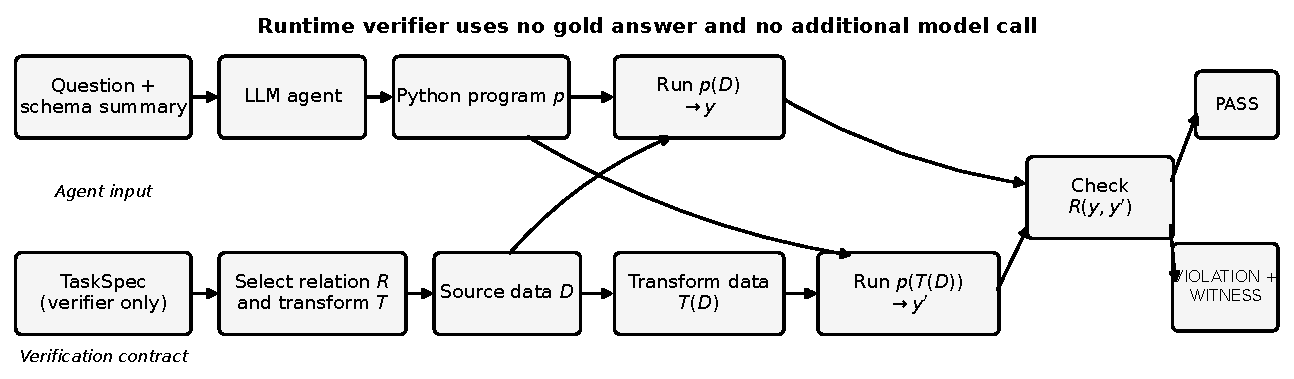
\includegraphics[width=0.98\textwidth]{figures/overview.pdf}
  \caption{\morph separates program generation from verification. The agent receives only the question and schema summary. The verifier receives the candidate program and a structured task specification, generates deterministic follow-up tables, re-executes the unchanged program, and checks the expected output relation. No gold answer or additional LLM call is used during verification.}
  \label{fig:overview}
\end{figure*}

Our contributions are:
\begin{enumerate}[leftmargin=*,itemsep=1pt,topsep=2pt]
  \item \textbf{A mutation-grounded verification benchmark.} We provide 101 compositional analytical tasks and 563 validated non-equivalent mutants across aggregation, filtering, grouping, ranking, and hardcoding faults.
  \item \textbf{Operator-aware, environment-grounded verification.} More than 20 relations transform the underlying data and check invariance, equivariance, monotonicity, or a forced counterfactual outcome without exposing the gold answer.
  \item \textbf{An accidental-correct evaluation protocol.} We hold each generated program fixed and re-execute it on held-out data distributions, revealing a substantial gap between single-seed and structural correctness.
  \item \textbf{Controlled and natural-agent evidence.} We report mutation coverage, natural-program precision/recall and accepted-answer risk, multi-transformation sensitivity, and a paired one-step repair study.
\end{enumerate}

\section{Related Work}
\label{sec:related}

\paragraph{Data-analysis agents and benchmarks.}
InfiAgent-DABench evaluates end-to-end analysis over CSV files \citep{hu2024infiagent}. DS-1000 and DSCodeBench test data-science code generation \citep{lai2022ds1000,ouyang2025dscodebench}. Recent benchmarks broaden coverage to agentic workflows, heterogeneous workspaces, and end-to-end computer environments \citep{zhang2025datascibench,nam2026dsstar,li2026dataspace,sun2026agenticdatabench,rahman2026dsagentbench}. These works primarily score final task success. \morph instead evaluates whether an execution-grounded verifier detects semantic faults, including programs that happen to return the correct output on one dataset.

\paragraph{Metamorphic and mutation testing.}
Metamorphic testing validates necessary relationships across transformed inputs when a direct test oracle is unavailable \citep{segura2016survey}. Mutation testing injects controlled faults to quantify a test suite's sensitivity \citep{jia2011mutation,petrovic2021mutation}. Prior work applies metamorphic transformations to text-to-SQL systems and language models \citep{ma2020mtteql,yang2025sqlhd,cho2025llmorph}. \morph differs in three ways: it transforms the \emph{tabular data environment} while keeping the candidate program fixed (rather than mutating the query or prompt); it activates relations only when the task specification warrants a particular analytical operator (e.g., a duplication test fires only for sum or mean metrics, not for every program); and it uses a validated semantic-mutant corpus to quantify how much of the fault space each relation family covers. This last property is consequential: a program using the wrong aggregation function can coincidentally return the correct ranking label on one dataset, and mutation scoring measures the fraction of such faults a verifier can detect via data-state transformations alone.

\paragraph{Verification signals for agents.}
Model-based judges and self-critique can inspect a trace, but they introduce an additional model call and may share the generator's semantic blind spots. \morph supplies a deterministic, falsifiable signal: a specific transformed dataset and pair of outputs that violate a declared relation. It is complementary to model-based judging rather than a replacement for it.

\section{Problem Setting}
\label{sec:problem}

A task is $t=(q,D,s)$, where $q$ is a natural-language question, $D$ is a dictionary of DataFrames, and $s$ is a structured analytical specification. The agent sees $q$ and a schema summary, and produces a reusable program $p$ implementing \texttt{analyze(tables)}. The verifier sees $p$ and $s$, but not a reference program or gold output.

The source result is $y=p(D)$. A metamorphic test $m=(T,R)$ contains a deterministic data transformation $T$ and a necessary output relation $R$. It produces $D'=T(D)$ and $y'=p(D')$. A violation is
\begin{equation}
  v_m(p,t)=\mathbf{1}\!\left[\neg R_m(y,y')\right].
\end{equation}
The program is flagged if any applicable relation violates. Relations express equality, known scaling, monotonic change, or a forced winner. Passing all relations is not proof of correctness: each relation encodes only a necessary condition.

For controlled evaluation, a semantic mutant is \emph{killed} when at least one relation flags it. Mutation score is the fraction of validated, non-equivalent mutants killed. For natural programs, we report precision, recall, false-positive rate (FPR), and accepted-answer risk $\mathrm{AAR}=\mathrm{FN}/(\mathrm{FN}+\mathrm{TN})$, the probability that an accepted executable program is wrong.

\section{MORPH-DA}
\label{sec:method}

\subsection{Specification-conditioned relation library}

Each \taskSpec records filters, metric operators, grouping dimensions, date windows, ranking direction, comparison periods, and output type. The natural-language question is generated from this specification, but the agent never receives the specification itself. This separation lets the benchmark test whether an agent inferred and implemented the requested computation, while the verifier checks compliance without knowing the numeric answer.

Relations are activated only when their premises are justified by the specification. Representative families are:

\begin{itemize}[leftmargin=*,itemsep=1pt,topsep=2pt]
  \item \textbf{Universal robustness:} row permutation and column-order invariance detect accidental positional dependence.
  \item \textbf{Filter and scope:} inject extreme rows that violate a required filter; a correct program must ignore them. A complementary in-scope sentinel can be constructed to force a winner.
  \item \textbf{Aggregation and statistics:} full duplication preserves means, medians, distinct counts, ratios, and rankings but scales sums and counts. Non-median extreme perturbations distinguish mean from median. Translation, scaling, and count-vs-distinct checks provide additional operator-specific tests.
  \item \textbf{Grouping and ranking:} counterfactual group construction, rank reversal, and top-$k$ consistency expose wrong grouping dimensions, ascending/descending errors, and hardcoded labels.
  \item \textbf{Time and period comparisons:} period-isolated injections and a forced year-over-year winner expose swapped periods, missing date windows, and absolute-vs-relative change errors.
\end{itemize}

The current library supports sum, mean, median, count, distinct count, min, max, standard deviation, variance, quantile, ratio, percentage change, and correlation. Fields for weighted means and joins exist in the specification DSL, but no weighted-mean or join relations are implemented or evaluated in the present corpus.

\subsection{Counterexample witnesses and repair}
When a relation fails, the verifier records the transformation, source output, follow-up output, expected relation, and likely fault family. This record is a concrete counterexample rather than an opaque confidence score. In the repair experiment, the same base program is paired across four feedback strategies: no retry, generic feedback, the violated relation name, and a full witness.

\subsection{Multi-transformation sensitivity}
Many transformations contain randomized but deterministic choices, such as which eligible rows become sentinels. Running a second verifier random seed generates a different set of follow-up tables while keeping the candidate program and source data fixed. We use this as a sensitivity analysis, not as a uniformly preferred deployment mode, because additional tests can increase both recall and false positives.

\section{Benchmark Construction}
\label{sec:benchmark}

\paragraph{Tasks and data.}
The benchmark contains 101 single-table tasks over eight synthetic business scenarios: retail orders, web sessions, seller marketplace, SaaS subscriptions, marketing campaigns, payments, fulfillment, and customer support. Tasks span five compositional levels: scalar aggregation (24), grouped ranking (48), ratios or support thresholds (11), year-over-year comparison (16), and multi-filter ratio-plus-comparison tasks (2). Data generators include heavy-tailed metrics, nulls, duplicates, and current/prior periods. The same schema and question are retained while seeds change the underlying distribution.

\paragraph{Filter discriminability.}
For each required filter, we verify that applying it changes the gold answer on seeds 7, 42, and 123. Three tasks fail this discriminability check and are excluded from the 98-task cross-seed evaluation set; otherwise, a program omitting the filter could pass regardless of implementation.

\paragraph{Reference compiler and consistency.}
A structural compiler translates each \taskSpec into a Pandas reference program. All references execute on seeds 7, 42, and 123 and pass applicable relations. Because references and relations are co-developed from the same specification, this establishes benchmark internal consistency, not an independent zero-FPR estimate. Independent false-positive behavior is measured on LLM-generated programs.

\paragraph{Mutation funnel.}
AST operators generate 3,030 candidate mutations. Applicability, syntax, execution, and output-contract filters leave 709 candidates for equivalence testing. Across five oracle seeds, 146/709 (20.6\%) are equivalent and removed, yielding 563 validated non-equivalent mutants: 131 aggregation, 173 filter, 21 grouping, 129 hardcoding, and 109 ranking faults.

\section{Experiments}
\label{sec:experiments}

\paragraph{Agents.}
A LangGraph code agent generates one Python program per task from the question and schema summary using Claude Haiku 4.5, Sonnet 4.6, or Opus 4.5. Evaluation centers on the 101 seed-42 programs per model. The framework is an implementation substrate, not part of the claimed method.

\paragraph{Three evaluation conditions.}
Condition A uses seed-42 gold labels on all 101 tasks and therefore treats accidental corrects as correct. Condition B saves each seed-42 program and re-executes that exact source unchanged on seeds 7 and 123; failure on either reclassifies it as wrong. Conditions B and C use the 98 filter-discriminating tasks. Condition C retains the same corrected ground truth but runs \morph with two transformation seeds instead of one. Precision, recall, and FPR exclude original execution failures; their counts are reported separately.

\paragraph{Statistics.}
We use continuity-corrected McNemar tests for paired detector comparisons, Holm correction across the three natural-agent comparisons, and a task-clustered bootstrap with 3,000 resamples for confidence intervals. The mutation confidence interval also clusters by base task to avoid treating multiple mutants of one task as independent.

\section{Results}
\label{sec:results}

\subsection{Controlled semantic faults}

\begin{table}[t]
\centering
\caption{Detection on 563 validated, non-equivalent mutants. The intermediate configuration is a genuine run recorded alongside the full result.}
\label{tab:mutants}
\small
\begin{tabular}{lrrr}
\toprule
Verifier & Killed & Score & 95\% CI \\
\midrule
Execution only & 0 & 0.0\% & -- \\
Universal relations & 9 & 1.6\% & -- \\
\makecell[l]{Universal + filter\\+ aggregation} & 346 & 61.5\% & -- \\
\textbf{Full \morph} & \textbf{364} & \textbf{64.7\%} & \textbf{[58.4, 70.5]} \\
\bottomrule
\end{tabular}
\end{table}

\tabref{tab:mutants} shows that execution detects none of the semantic mutants, while universal row/column robustness checks kill only 9. Operator-conditioned relations account for the gain: full \morph kills 364 mutants ($\chi^2=353$, $n_{01}=355$, $n_{10}=0$, $p=9.4\times10^{-79}$). Filter and aggregation relations produce 346 kills; grouping, hardcoding, time, and statistical relations add 18. Thus the approximately $40\times$ ratio over universal checks primarily quantifies how weak non-semantic robustness tests are for operator faults.

\begin{figure}[t]
  \centering
  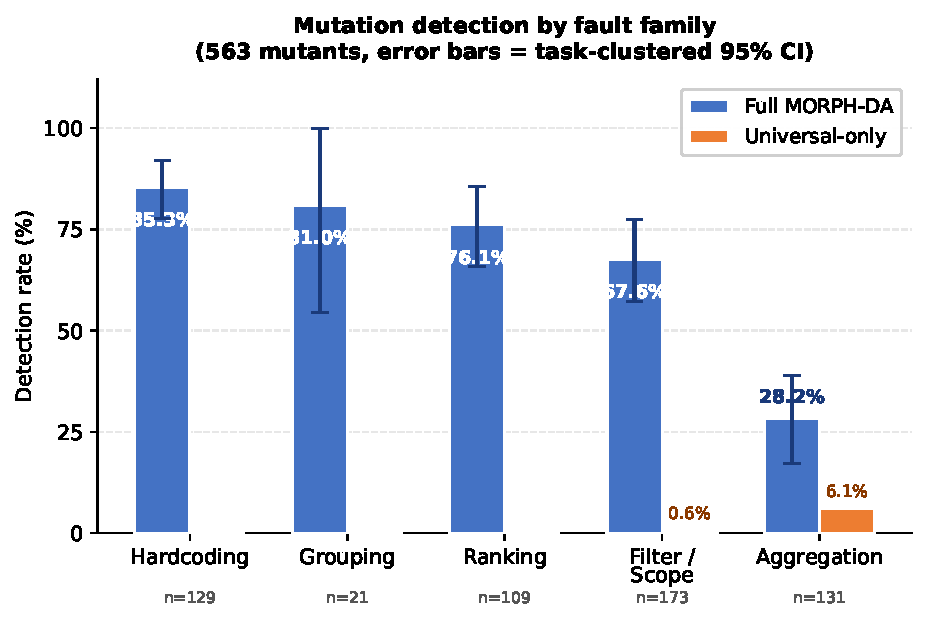
\includegraphics[width=\columnwidth]{figures/fault_family_detection.pdf}
  \caption{Mutation detection by fault family. Aggregation is hardest because a wrong aggregation can preserve the winning label on ranking tasks. Error bars are task-clustered 95\% bootstrap intervals.}
  \label{fig:families}
\end{figure}

Detection varies by family (\figref{fig:families}): hardcoding 85.3\%, grouping 81.0\%, ranking 76.1\%, filtering 67.6\%, and aggregation 28.2\%. Low aggregation coverage is partly unidentifiability: if both sum and mean select the same top group, no output-only relation can distinguish them on that instance.

\subsection{Accidental correctness}

On seed 42, 61/101 Haiku, 65/101 Sonnet, and 62/101 Opus programs appear correct. Re-executing those same programs unchanged on held-out seeds reduces structurally correct counts to 45, 52, and 49 (\figref{fig:accidental}). Therefore, 16, 13, and 13 programs -- 26.2\%, 20.0\%, and 21.0\% of apparent successes -- are accidental corrects. Without seeing held-out seeds, single-seed \morph catches 13/16 (81\%), 7/13 (54\%), and 10/13 (77\%) of them.

Manual inspection of the accidental-correct programs reveals three recurring failure modes. The dominant pattern is a \textbf{missing status or eligibility filter}: the program omits or substitutes the required row-level condition (e.g., applying \texttt{notna()} as a proxy for \texttt{status~!=~`open'}, or filtering for \texttt{status~!=~`returned'} when \texttt{status~!=~`cancelled'} is required), and the excluded segment happens not to shift the ranking winner on the seed-42 distribution. A second pattern is \textbf{elided date scope}: the program skips the required date window entirely and the dominant group is the same across historical data as within the target period. A third pattern appears in year-over-year and quarterly tasks: the program implements the correct temporal structure but omits a required status filter; because the excluded segment is proportionally similar across both periods on seed~42, the ranking winner is preserved. \morph detects the first two categories primarily through MR-F1 (filter injection) and MR-T (time scope) relations; the third is harder to detect because the filter omission is symmetric across periods and produces no observable difference under single-seed transformation.

\begin{figure}[t]
  \centering
  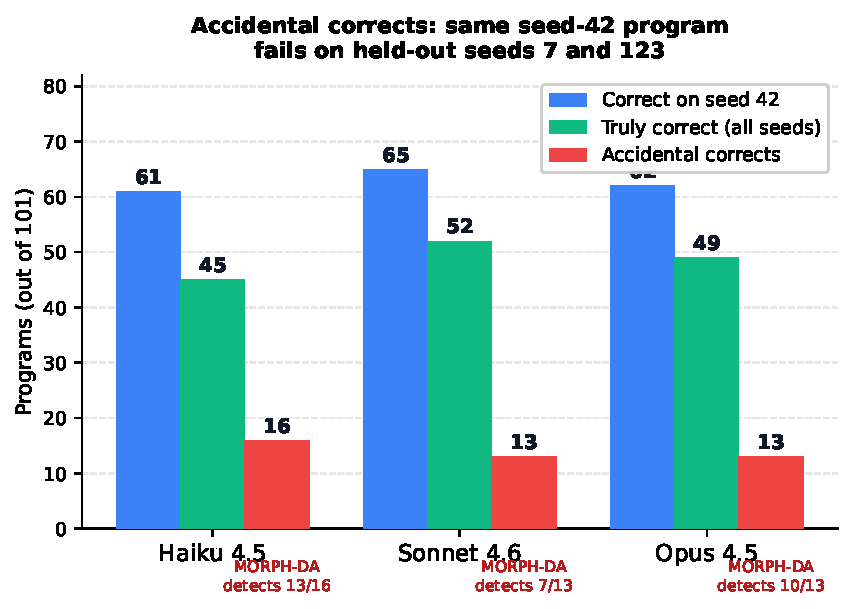
\includegraphics[width=\columnwidth]{figures/accidental_corrects.pdf}
  \caption{Programs correct on seed 42 split into truly correct and accidental correct after fixed-program re-execution on seeds 7 and 123.}
  \label{fig:accidental}
\end{figure}

\subsection{Natural-program verification}

\begin{table*}[t]
\centering
\caption{Natural-program verification. Condition A uses 101 tasks and naive seed-42 labels. Conditions B/C use the 98-task filter-discriminating set and cross-seed corrected labels. Original execution failures (Haiku 2, Sonnet 0, Opus 2) are excluded from precision/recall/FPR denominators. CIs shown for the primary Condition B.}
\label{tab:natural}
\small
\begin{adjustbox}{max width=\textwidth}
\begin{tabular}{llrrrrr}
\toprule
Model & Condition & Precision & Recall & FPR & F1 & AAR \\
\midrule
\multirow{3}{*}{Haiku 4.5}
 & A: naive & 58.8 & 79.0 & 34.4 & 67.4 & 16.7 \\
 & \textbf{B: cross-seed} & \textbf{87.5} [77.1,95.8] & \textbf{79.2} [67.9,90.6] & \textbf{14.0} [4.7,25.6] & 83.2 & 22.9 \\
 & C: two transformations & 86.0 & 81.1 & 16.3 & 83.5 & 21.7 \\
\midrule
\multirow{3}{*}{Sonnet 4.6}
 & A: naive & 66.7 & 72.2 & 20.0 & 69.3 & 16.1 \\
 & \textbf{B: cross-seed} & \textbf{89.2} [78.4,97.3] & \textbf{67.3} [53.1,79.6] & \textbf{8.2} [2.0,18.4] & 76.7 & 26.2 \\
 & C: two transformations & 86.8 & 67.3 & 10.2 & 75.9 & 26.7 \\
\midrule
\multirow{3}{*}{Opus 4.5}
 & A: naive & 58.8 & 81.1 & 33.9 & 68.2 & 14.6 \\
 & \textbf{B: cross-seed} & \textbf{79.2} [68.8,89.6] & \textbf{79.2} [66.7,89.6] & \textbf{20.8} [10.4,33.3] & 79.2 & 20.8 \\
 & C: two transformations & 78.0 & 81.2 & 22.9 & 79.6 & 19.6 \\
\bottomrule
\end{tabular}
\end{adjustbox}
\end{table*}

Under naive labels, correctly flagged accidental programs are counted as false positives, depressing apparent precision to 59--67\%. With fixed-program cross-seed ground truth, Condition B obtains 79--89\% precision and 67--79\% recall (\tabref{tab:natural}). Against universal-only relations, the full verifier adds 37--48 true detections and loses none (Holm-corrected $p\leq3.25\times10^{-9}$ for all models). False positives remain nontrivial: 8.2--20.8\%, driven mainly by extreme filter injections, tie-sensitive forced-group tests, and legal computed constants flagged by the hardcoding relation.

A second transformation seed changes recall by +1.9, 0.0, and +2.1 percentage points for Haiku, Sonnet, and Opus, while increasing FPR by about 2 points for each model. It slightly improves F1 for Haiku and Opus but lowers it for Sonnet. Condition C is therefore a multi-transformation sensitivity analysis rather than a default; deployments that value recall over false alarms may choose it.

\subsection{One-step repair}

\begin{table}[t]
\centering
\caption{Paired one-step repair on 91 wrong-but-executable Haiku programs from seeds 7, 42, and 123.}
\label{tab:repair}
\small
\begin{tabular}{llrr}
\toprule
ID & Feedback & Fixed & Rate \\
\midrule
R0 & No retry & 0/91 & 0.0\% \\
R2 & Generic ``has a bug'' & 5/91 & 5.5\% \\
R6 & Violated relation name & 11/91 & 12.1\% \\
R7 & Full counterexample witness & 11/91 & 12.1\% \\
\bottomrule
\end{tabular}
\end{table}

The 91-program sample spans seeds 7 (25 programs), 42 (38), and 123 (28), covering 55 distinct tasks. Relation-name and witness feedback each produce 11/91 fixes versus 5/91 for generic feedback (\tabref{tab:repair}). For each comparison with R2, $n_{01}=6$ and $n_{10}=0$ ($p=0.041$ unadjusted; $p=0.082$ after Holm correction for two co-primary comparisons), so we report a higher observed rate rather than a superiority claim. R6 and R7 have the same aggregate rate but repair different programs ($n_{01}=4$, $n_{10}=4$, $p=0.29$); the study does not establish that a richer one-step witness is better than the relation name alone.

\paragraph{Runtime cost.}
Verification adds no model calls. In a 20-task reference-program pilot measured with raw Python timer timestamps, the full relation set required approximately 40 Python executions per task and had 500\,ms mean, 525\,ms median, and 1.14\,s p95 runtime. This is a small pilot, not a production latency claim.

\section{Limitations and Discussion}
\label{sec:limitations}

\paragraph{Specification dependence.}
\morph assumes a structured analytical specification. Such specifications may be authored by analysts, derived from governed metric definitions, or extracted by a separate model; automatic extraction and verification of the specification itself are outside scope. The method is gold-answer-free, not supervision-free.

\paragraph{Incomplete necessary conditions.}
Passing the current relations does not prove correctness. Aggregation coverage is especially limited on label-output tasks when wrong operators preserve the winner. New relation families, richer output contracts, and combinations with learned judges may improve recall.

\paragraph{Benchmark and model scope.}
The evaluated data are synthetic, all tasks are single-table, and all natural programs come from three variants of one model family using a LangGraph harness. Join and weighted-mean fields are represented in the DSL, but neither capability has implemented relations or evaluated tasks. Generalization to open-weight models, SQL, multi-table analysis, and real enterprise datasets remains to be tested. We note that the task structures and analytical operators---scalar aggregation, grouped ranking, period-over-period comparison, and filtered ratio---reflect query patterns common in enterprise analytics workflows. The synthetic generator and task set were finalized before natural-agent evaluation began; observed LLM failure modes were not used to tune task difficulty or filter coverage, avoiding circularity between task design and measurement.

\paragraph{Reference and repair limitations.}
Reference programs and relations share the same specifications, so reference pass rates measure internal consistency rather than an independent FPR. Natural-agent programs provide the independent FPR estimate. Finally, repair success is low and one-step only; equal aggregate R6/R7 rates and non-significant paired differences motivate multi-round and fault-specific repair studies.

\paragraph{Implications for agent verification.}
The main lesson is not that metamorphic testing replaces gold evaluation. Instead, it supplies a reusable environment-grounded signal where direct answers are unavailable, exposes single-instance accidental correctness, and creates counterexamples that can support debugging, model-based judging, or human review.

\section{Conclusion}

Execution success is an inadequate verifier for analytical agents, and single-instance correctness can conceal structurally wrong programs. \morph combines a mutation-grounded benchmark with specification-conditioned data transformations to test necessary behavioral properties without revealing the gold output. It detects 64.7\% of 563 semantic mutants, identifies a substantial fraction of accidental corrects, and yields useful precision/recall tradeoffs on natural agent programs without an additional LLM verification call. The remaining false positives and undetected aggregation errors reinforce the intended interpretation: metamorphic execution is a complementary runtime verifier, not a correctness certificate.

\bibliographystyle{plainnat}
\bibliography{references}

\clearpage
\appendix

\section{Additional Experimental Detail}

\subsection{Condition-B confusion matrices}
\begin{table}[h]
\centering
\caption{Cross-seed corrected confusion matrices. Original execution failures are excluded.}
\small
\begin{tabular}{lrrrrr}
\toprule
Model & TP & FP & TN & FN & Evaluated \\
\midrule
Haiku 4.5 & 42 & 6 & 37 & 11 & 96 \\
Sonnet 4.6 & 33 & 4 & 45 & 16 & 98 \\
Opus 4.5 & 38 & 10 & 38 & 10 & 96 \\
\bottomrule
\end{tabular}
\end{table}

\subsection{Seed-42 execution breakdown}
\begin{table}[h]
\centering
\caption{Original seed-42 program outcomes on the 98-task filter-discriminating set.}
\small
\begin{tabular}{lrrr}
\toprule
Model & Correct & Wrong executable & Execution failure \\
\midrule
Haiku 4.5 & 59 & 37 & 2 \\
Sonnet 4.6 & 62 & 36 & 0 \\
Opus 4.5 & 61 & 35 & 2 \\
\bottomrule
\end{tabular}
\end{table}

\subsection{Relation-level false positives}
\begin{table}[h]
\centering
\caption{Condition-B false positives by dominant relation.}
\small
\begin{tabularx}{\columnwidth}{lrrrX}
\toprule
Relation & Haiku & Sonnet & Opus & Typical cause \\
\midrule
MR-F1 & 4 & 2 & 6 & Imprecise filter logic under extreme rows \\
MR-G3 & 1 & 1 & 2 & Tie-break sensitivity \\
MR-H1 & 1 & 1 & 2 & Legal computed constants \\
\bottomrule
\end{tabularx}
\end{table}

\subsection{Mutant-generation funnel}
The verified funnel is $3{,}030 \rightarrow 709 \rightarrow 563$: generated candidates, executable candidates entering equivalence evaluation, and retained non-equivalent mutants, respectively. Of the 709 executable candidates, 146 (20.6\%) were equivalent across five oracle seeds and removed. An intermediate \texttt{rulemut\_stats.json} file from an earlier run is not used for final results.

\subsection{Repair pairing and provenance}
The repair log contains 364 rows: 91 source programs crossed with four strategies. Each row includes a stable program identifier, model, data seed, and source hash, enabling row-paired comparisons. The source-program distribution is 25 programs from seed 7, 38 from seed 42, and 28 from seed 123.

\subsection{Reproducibility and anonymity}
The anonymous supplementary package contains task specifications, data generators, relation implementations, evaluation scripts, aggregate result tables, and de-identified logs. Public author-identifying repository links are intentionally omitted during double-blind review.

\end{document}
